\renewcommand*{\arraystretch}{1.1}

\subsection*{BI / read / 2}
\label{section:bi-read-02}

% change \emph{} to use sans-serif font
\let\oldemph\emph
\renewcommand{\emph}[1]{{\footnotesize \sf #1}}

\renewcommand{\currentQueryCard}{2}
\marginpar{
	\raggedleft
	\vspace{0.22ex}

	\queryRefCard{bi-read-01}{BI}{1}\\
	\queryRefCard{bi-read-02}{BI}{2}\\
	\queryRefCard{bi-read-03}{BI}{3}\\
	\queryRefCard{bi-read-04}{BI}{4}\\
	\queryRefCard{bi-read-05}{BI}{5}\\
	\queryRefCard{bi-read-06}{BI}{6}\\
	\queryRefCard{bi-read-07}{BI}{7}\\
	\queryRefCard{bi-read-08}{BI}{8}\\
	\queryRefCard{bi-read-09}{BI}{9}\\
	\queryRefCard{bi-read-10}{BI}{10}\\
	\queryRefCard{bi-read-11}{BI}{11}\\
	\queryRefCard{bi-read-12}{BI}{12}\\
	\queryRefCard{bi-read-13}{BI}{13}\\
	\queryRefCard{bi-read-14}{BI}{14}\\
	\queryRefCard{bi-read-15}{BI}{15}\\
	\queryRefCard{bi-read-16}{BI}{16}\\
	\queryRefCard{bi-read-17}{BI}{17}\\
	\queryRefCard{bi-read-18}{BI}{18}\\
	\queryRefCard{bi-read-19}{BI}{19}\\
	\queryRefCard{bi-read-20}{BI}{20}\\
	\queryRefCard{bi-read-21}{BI}{21}\\
	\queryRefCard{bi-read-22}{BI}{22}\\
	\queryRefCard{bi-read-23}{BI}{23}\\
	\queryRefCard{bi-read-24}{BI}{24}\\
	\queryRefCard{bi-read-25}{BI}{25}\\
}


\noindent\begin{tabularx}{\queryCardWidth}{|>{\queryPropertyCell}p{\queryPropertyCellWidth}|X|}
	\hline
	query & BI / read / 2 \\ \hline
%
	title & Top tags for country, age, gender, time \\ \hline
%
	pattern & \hfill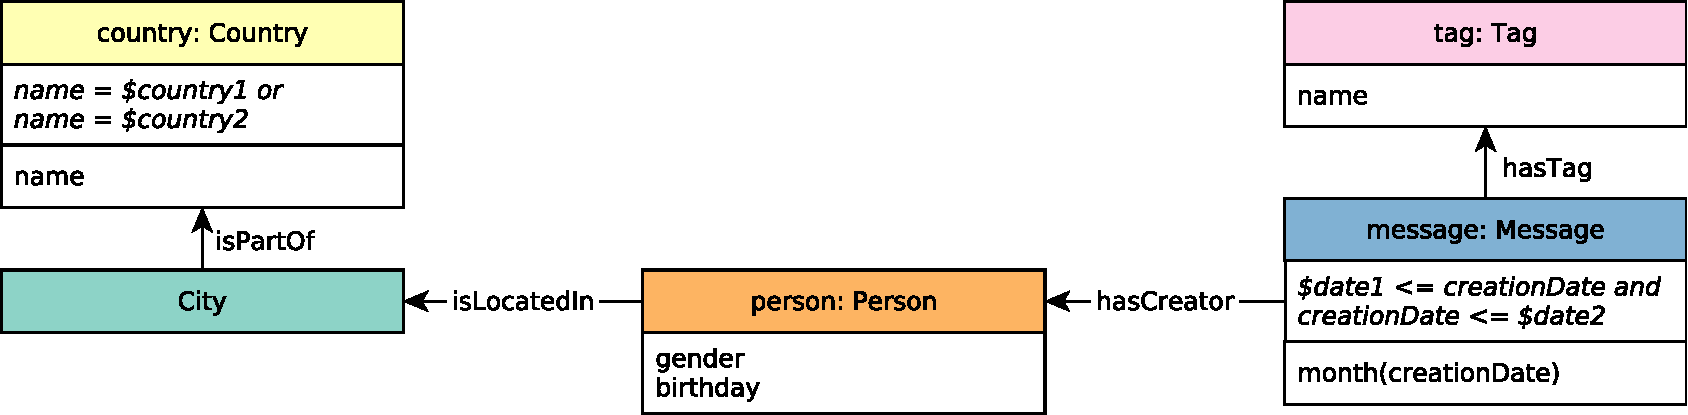
\includegraphics[scale=\patternscale,margin=0cm .2cm]{patterns/bi-read-02}\hfill\vadjust{} \\ \hline
%
	desc. & Select all \emph{Messages} created in the range of
\texttt{{[}startDate,\ endDate{]}} by \emph{Persons} located in
\texttt{country1} or \texttt{country2}. Select the creator
\emph{Persons} and the \emph{Tags} of these \emph{Messages}. Split these
\emph{Persons}, \emph{Tags} and \emph{Messages} into a 5-level grouping:

\begin{enumerate}
\def\labelenumi{\arabic{enumi}.}
\tightlist
\item
  name of country of \emph{Person},
\item
  month the \emph{Message} was created,
\item
  gender of \emph{Person},
\item
  age group of \emph{Person}, defined as years between person's birthday
  and end of simulation (2013-01-01), divided by 5, rounded down
  (partial years do not count),
\item
  name of tag attached to \emph{Message}.
\end{enumerate}

Consider only those groups where number of \emph{Messages} is greater
than 100.
 \\ \hline
%
	
		params &
		\innerCardVSpace{\begin{tabularx}{\attributeCardWidth}{|>{\paramNumberCell}c|>{\varNameCell}M|>{\typeCell}m{\typeWidth}|Y|} \hline
		$\mathsf{1}$ & startDate
 & Date
 &  \\ \hline
		$\mathsf{2}$ & endDate
 & Date
 &  \\ \hline
		$\mathsf{3}$ & country1
 & String
 &  \\ \hline
		$\mathsf{4}$ & country2
 & String
 &  \\ \hline
		\end{tabularx}}\innerCardVSpace \\ \hline
	
%
	
		result &
		\innerCardVSpace{\begin{tabularx}{\attributeCardWidth}{|>{\resultNumberCell}c|>{\varNameCell}M|>{\typeCell}m{\typeWidth}|>{\resultOriginCell}c|Y|} \hline
		$\mathsf{1}$ & country.name & String & R &
				 \\ \hline
		$\mathsf{2}$ & messageMonth & 32-bit Integer & R &
				1--12
 \\ \hline
		$\mathsf{3}$ & person.gender & String & R &
				\texttt{male}/\texttt{female}
 \\ \hline
		$\mathsf{4}$ & ageGroup & 32-bit Integer & C &
				 \\ \hline
		$\mathsf{5}$ & tag.name & String & R &
				 \\ \hline
		$\mathsf{6}$ & messageCount & 64-bit Integer & A &
				The number of messages in the group
 \\ \hline
		\end{tabularx}}\innerCardVSpace \\ \hline
	
%
	
		sort		&
		\innerCardVSpace{\begin{tabularx}{\attributeCardWidth}{|>{\sortNumberCell}c|>{\varNameCell}M|>{\directionCell}c|Y|} \hline
		$\mathsf{1}$ & messageCount
 & $\desc
$ &  \\ \hline
		$\mathsf{2}$ & tag.name
 & $\asc
$ &  \\ \hline
		$\mathsf{3}$ & ageGroup
 & $\asc
$ &  \\ \hline
		$\mathsf{4}$ & person.gender
 & $\asc
$ &  \\ \hline
		$\mathsf{5}$ & messageMonth
 & $\asc
$ &  \\ \hline
		$\mathsf{6}$ & country.name
 & $\asc
$ &  \\ \hline
		\end{tabularx}}\innerCardVSpace \\ \hline
	%
	limit & 100 \\ \hline
	%
	CPs &
	\multicolumn{1}{>{\raggedright}l|}{
		\chokePoint{1.1}, 
		\chokePoint{1.2}, 
		\chokePoint{1.4}, 
		\chokePoint{2.1}, 
		\chokePoint{2.3}, 
		\chokePoint{3.1}, 
		\chokePoint{3.2}
		} \\ \hline
	%
	%
\end{tabularx}
\queryCardVSpace

% change \emph back to the old one
\renewcommand{\emph}[1]{\oldemph{#1}}